%package list
\documentclass{article}
\usepackage[top=3cm, bottom=3cm, outer=3cm, inner=3cm]{geometry}
\usepackage{multicol}
\usepackage{graphicx}
\usepackage{url}
%\usepackage{cite}
\usepackage{hyperref}
\usepackage{array}
%\usepackage{multicol}
\newcolumntype{x}[1]{>{\centering\arraybackslash\hspace{0pt}}p{#1}}
\usepackage{natbib}
\usepackage{pdfpages}
\usepackage{multirow}
\usepackage[normalem]{ulem}
\useunder{\uline}{\ul}{}
\usepackage{svg}
\usepackage{xcolor}
\usepackage{listings}
\lstdefinestyle{ascii-tree}{
    literate={├}{|}1 {─}{--}1 {└}{+}1 
  }
\lstset{basicstyle=\ttfamily,
  showstringspaces=false,
  commentstyle=\color{red},
  keywordstyle=\color{blue}
}
%\usepackage{booktabs}
\usepackage{caption}
\usepackage{subcaption}
\usepackage{float}
\usepackage{array}

\newcolumntype{M}[1]{>{\centering\arraybackslash}m{#1}}
\newcolumntype{N}{@{}m{0pt}@{}}


%%%%%%%%%%%%%%%%%%%%%%%%%%%%%%%%%%%%%%%%%%%%%%%%%%%%%%%%%%%%%%%%%%%%%%%%%%%%
%%%%%%%%%%%%%%%%%%%%%%%%%%%%%%%%%%%%%%%%%%%%%%%%%%%%%%%%%%%%%%%%%%%%%%%%%%%%
\newcommand{\itemEmail}{dhuamanio@unsa.edu.pe}
\newcommand{\itemStudent}{David Alfredo Huamani Ollachica}
\newcommand{\itemCourse}{Programación Web 2}
\newcommand{\itemCourseCode}{1702122}
\newcommand{\itemSemester}{III}
\newcommand{\itemUniversity}{Universidad Nacional de San Agustín de Arequipa}
\newcommand{\itemFaculty}{Facultad de Ingeniería de Producción y Servicios}
\newcommand{\itemDepartment}{Departamento Académico de Ingeniería de Sistemas e Informática}
\newcommand{\itemSchool}{Escuela Profesional de Ingeniería de Sistemas}
\newcommand{\itemAcademic}{2024 - A}
\newcommand{\itemInput}{Del 17 Mayo 2024}
\newcommand{\itemOutput}{Al 18 Mayo 2024}
\newcommand{\itemPracticeNumber}{03}
\newcommand{\itemTheme}{JavaScript}
%%%%%%%%%%%%%%%%%%%%%%%%%%%%%%%%%%%%%%%%%%%%%%%%%%%%%%%%%%%%%%%%%%%%%%%%%%%%
%%%%%%%%%%%%%%%%%%%%%%%%%%%%%%%%%%%%%%%%%%%%%%%%%%%%%%%%%%%%%%%%%%%%%%%%%%%%

\usepackage[english,spanish]{babel}
\usepackage[utf8]{inputenc}
\AtBeginDocument{\selectlanguage{spanish}}
\renewcommand{\figurename}{Figura}
\renewcommand{\refname}{Referencias}
\renewcommand{\tablename}{Tabla} %esto no funciona cuando se usa babel
\AtBeginDocument{%
	\renewcommand\tablename{Tabla}
}

\usepackage{fancyhdr}
\pagestyle{fancy}
\fancyhf{}
\setlength{\headheight}{30pt}
\renewcommand{\headrulewidth}{1pt}
\renewcommand{\footrulewidth}{1pt}
\fancyhead[L]{\raisebox{-0.2\height}{
\includegraphics[width=3cm]{img/logo_episunsa.png}}}
\fancyhead[C]{\fontsize{7}{7}\selectfont	\itemUniversity \\ \itemFaculty \\ \itemDepartment \\ \itemSchool \\ \textbf{\itemCourse}}
\fancyhead[R]{\raisebox{-0.2\height}{
\includegraphics[width=1.2cm]{img/logo_abet}}}
\fancyfoot[L]{Estudiante David Huamani Ollachica}
\fancyfoot[C]{\itemCourse}
\fancyfoot[R]{Página \thepage}

% para el codigo fuente
\usepackage{listings}
\usepackage{color, colortbl}
\definecolor{dkgreen}{rgb}{0,0.6,0}
\definecolor{gray}{rgb}{0.5,0.5,0.5}
\definecolor{mauve}{rgb}{0.58,0,0.82}
\definecolor{codebackground}{rgb}{0.95, 0.95, 0.92}
\definecolor{tablebackground}{rgb}{0.8, 0, 0}

\lstset{frame=tb,
	language=bash,
	aboveskip=3mm,
	belowskip=3mm,
	showstringspaces=false,
	columns=flexible,
	basicstyle={\small\ttfamily},
	numbers=none,
	numberstyle=\tiny\color{gray},
	keywordstyle=\color{blue},
	commentstyle=\color{dkgreen},
	stringstyle=\color{mauve},
	breaklines=true,
	breakatwhitespace=true,
	tabsize=3,
	backgroundcolor= \color{codebackground},
}

\begin{document}
	
	\vspace*{10px}
	
	\begin{center}	
		\fontsize{17}{17} \textbf{ Informe de Laboratorio \itemPracticeNumber}
	\end{center}
	\centerline{\textbf{\Large Tema: \itemTheme}}
	%\vspace*{0.5cm}	

	\begin{flushright}
		\begin{tabular}{|M{2.5cm}|N|}
			\hline 
			\rowcolor{tablebackground}
			\color{white} \textbf{Nota}  \\
			\hline 
			     \\[30pt]
			\hline 			
		\end{tabular}
	\end{flushright}	

	\begin{table}[H]
		\begin{tabular}{|x{4.7cm}|x{4.8cm}|x{4.8cm}|}
			\hline 
			\rowcolor{tablebackground}
			\color{white} \textbf{Estudiante} & \color{white}\textbf{Escuela}  & \color{white}\textbf{Asignatura}   \\
			\hline 
			{\itemStudent \par \itemEmail} & \itemSchool & {\itemCourse \par Semestre: \itemSemester \par Código: \itemCourseCode}     \\
			\hline 			
		\end{tabular}
	\end{table}		
	
	\begin{table}[H]
		\begin{tabular}{|x{4.7cm}|x{4.8cm}|x{4.8cm}|}
			\hline 
			\rowcolor{tablebackground}
			\color{white}\textbf{Laboratorio} & \color{white}\textbf{Tema}  & \color{white}\textbf{Duración}   \\
			\hline 
			\itemPracticeNumber & \itemTheme & 04 horas   \\
			\hline 
		\end{tabular}
	\end{table}
	
	\begin{table}[H]
		\begin{tabular}{|x{4.7cm}|x{4.8cm}|x{4.8cm}|}
			\hline 
			\rowcolor{tablebackground}
			\color{white}\textbf{Semestre académico} & \color{white}\textbf{Fecha de inicio}  & \color{white}\textbf{Fecha de entrega}   \\
			\hline 
			\itemAcademic & \itemInput &  \itemOutput  \\
			\hline 
		\end{tabular}
	\end{table}
	
	\section{Tarea}
	\begin{itemize}		
		\item Programar en JavaScript sobre una página web html básica.
		\item Ejercicio 01: Cree un teclado random para banca por internet.
		\item Ejercicio 02: Cree una calculadora básica como la de los sistemas operativos, que pueda utilizar
la función eval() y que guarde todos las operaciones en una pila. Mostrar la pila al píe de la página
web.
		\item Ejercicio 03: Cree una versión de el juego ’el ahorcado’ que grafique con canvas paso a paso
desde el evento onclick() de un botón.

	\end{itemize}
		
	\section{Equipos, materiales y temas utilizados}
	\begin{itemize}
		\item Sistema Operativo Ubuntu GNU Linux 23 lunar 64 bits Kernell 6.2.
		\item VIM 9.0.
		\item OpenJDK 64-Bits 17.0.7.
		\item Git 2.39.2.
		\item Cuenta en GitHub con el correo institucional.
		\item HTML, CSS y JavaScript
		\item DOM
	\end{itemize}
	
	\section{URL de Repositorio Github}
	\begin{itemize}
		\item URL para el laboratorio 03 en el Repositorio GitHub.
		\item \url{https://github.com/dev1d123/pw2_lab03}
	\end{itemize}
	        		\begin{figure}[H]
            \centering
            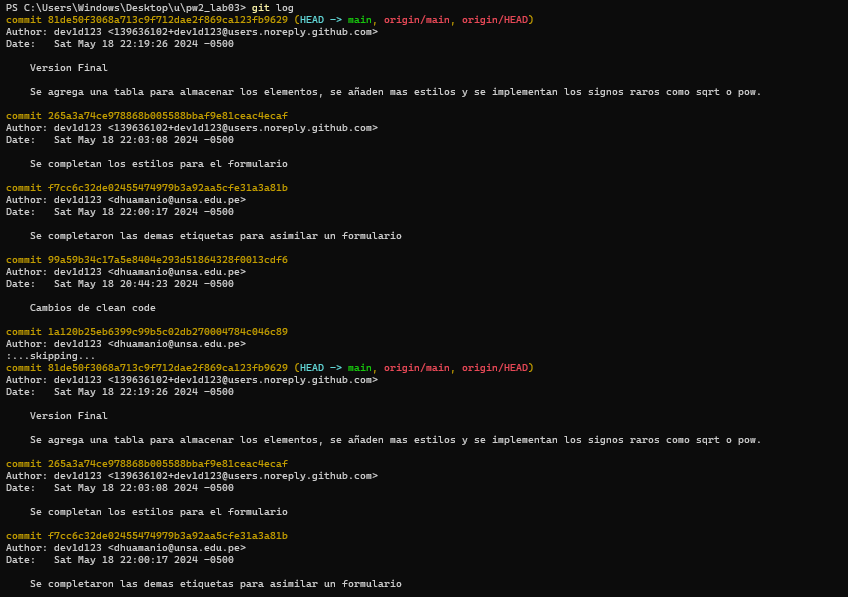
\includegraphics[width=\textwidth]{img/commit1}
            \caption{Imagen de los commits con git log}
            \label{fig:pagina}
        \end{figure}
        		\begin{figure}[H]
            \centering
            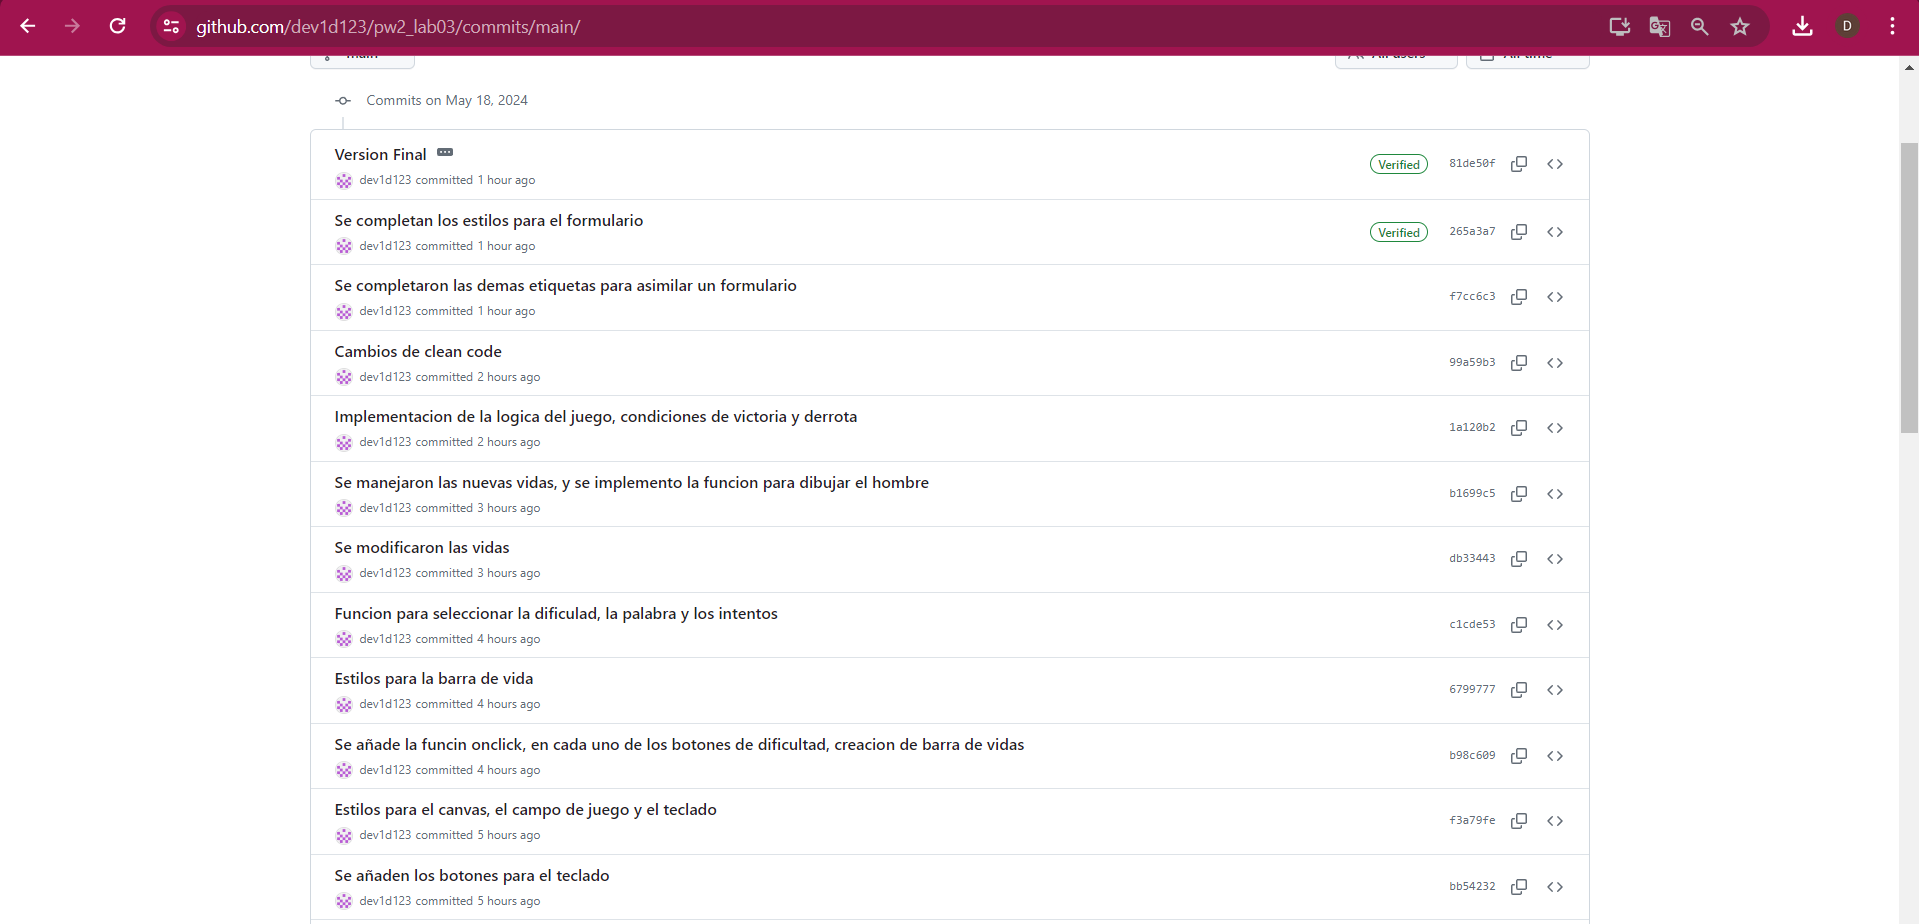
\includegraphics[width=\textwidth]{img/commit2}
            \caption{Imagen de los commits en el repositorio}
            \label{fig:pagina}
        \end{figure}

	\section{Ejercicios propuestos}
	
	\subsection{Ejercicio 1}
	\begin{itemize}	
		\item Documento HTML, se trato de imitar el formulario propuesto en la guia, a modo de practica, se añadireon los botones (button) con sus respectivas clases, debido a que se utilizara sus atributos text.content.
	\end{itemize}	
		
	\begin{lstlisting}[language=html,caption={Ejercicio1/index.html}][H]
<!DOCTYPE html>
<html lang="en">
<head>
    <meta charset="UTF-8">
    <meta name="viewport" content="width=device-width, initial-scale=1.0">
    <title>Formulario Bancario</title>
    <link rel="stylesheet" href="styles.css">
</head>
<body>
    <header>
        <h1>Formulario Bancario</h1>
    </header>
    <div class="form-container">
        <form action="#" method="post">
            <div class="form-group">
                <label for="bank">Banco:</label>
                <select name="bank" id="bank">
                    <option value="bpv">BPC</option>
                    <option value="interbank">Interbank</option>
                    <option value="scotiabank">Scotiabank</option>
                </select>
            </div>
            <div class="form-group">
                <label for="card-number">Numero de Tarjeta:</label>
                <input type="number" name="card-number" id="card-number" required>
            </div>
            <div class="form-group">
                <label>Tipo de DNI:</label>
                <label for="normal"><input type="radio" name="tipodni" id="normal" value="normal" checked> Normal</label>
                <label for="electronico"><input type="radio" name="tipodni" id="electronico" value="electronico"> Electronico</label>
            </div>
            <div class="form-group">
                <label for="dni-number">Numero de DNI:</label>
                <input type="number" name="dni-number" id="dni-number" required>
            </div>
            <div class="container">
                <input type="text" name="text" id="in" class="in" dir="rtl">
                <div class="buttons">
                    <button type="button" class="b">1</button>
                    <button type="button" class="b">2</button>
                    <button type="button" class="b">3</button>
                    <button type="button" class="b">4</button>
                    <button type="button" class="b">5</button>
                    <button type="button" class="b">6</button>
                    <button type="button" class="b">7</button>
                    <button type="button" class="b">8</button>
                    <button type="button" class="b">9</button>
                    <button type="button" class="b">0</button>
                    <button type="button" id="clear" class="big">Clear</button>
                </div>
            </div>
            <div class="form-group">
                <a href="#" class="forgot-password">Olvide mi contrasena</a>
            </div>
            <div class="form-group">
                <button type="submit" class="submit">Enviar</button>
            </div>
        </form>
    </div>

    <script src="script_ejercicio_01.js"></script>
</body>
</html>
	\end{lstlisting}
\begin{itemize}	
		\item Archivo JavaScript, se utiliza un set para la generacion de los numeros aleatorios, mediante una iteracion, luego se copian estos datos a un arreglo, posteriormente se distribuyen los elementos de este arreglo a todos los botones mediante un querySelectorAll.
	\end{itemize}	
		
	\begin{lstlisting}[language=html,caption={Ejercicio1/scriptejercicio01.js}][H]
console.log("Exito")
var elem = document.getElementsByTagName("body");
console.log(elem);
var random =Math.floor(Math.random()*10);
console.log("Numero aleatorio!", random);

var numerosAleatorios = new Set();

while(numerosAleatorios.size != 10){
    random =Math.floor(Math.random()*10);
    console.log("Numero aleatorio!", random);
    numerosAleatorios.add(random);
}
console.log(numerosAleatorios);
var arreglo = [];

numerosAleatorios.forEach(elem =>{
    arreglo.push(elem);
});

console.log(arreglo);

//obtener los elementos 
var buttons = document.querySelectorAll(".b");
console.log(buttons);
var index = 0;
buttons.forEach(b =>{
    b.textContent = arreglo[index];
    index++;
});

//agregando funcionalidad a los botones
var input = document.getElementById("in");
console.log(input);
buttons.forEach(b =>{
    b.addEventListener('click', function(){
        console.log("click", b.textContent);
        input.value = input.value + b.textContent;
    });
});


var cl = document.getElementById("clear");
cl.addEventListener('click', function(){
    input.value = "";
});
	\end{lstlisting}
	\begin{itemize}	
		\item Imagen de la pagina.
		
		
		
		\begin{figure}[H]
            \centering
            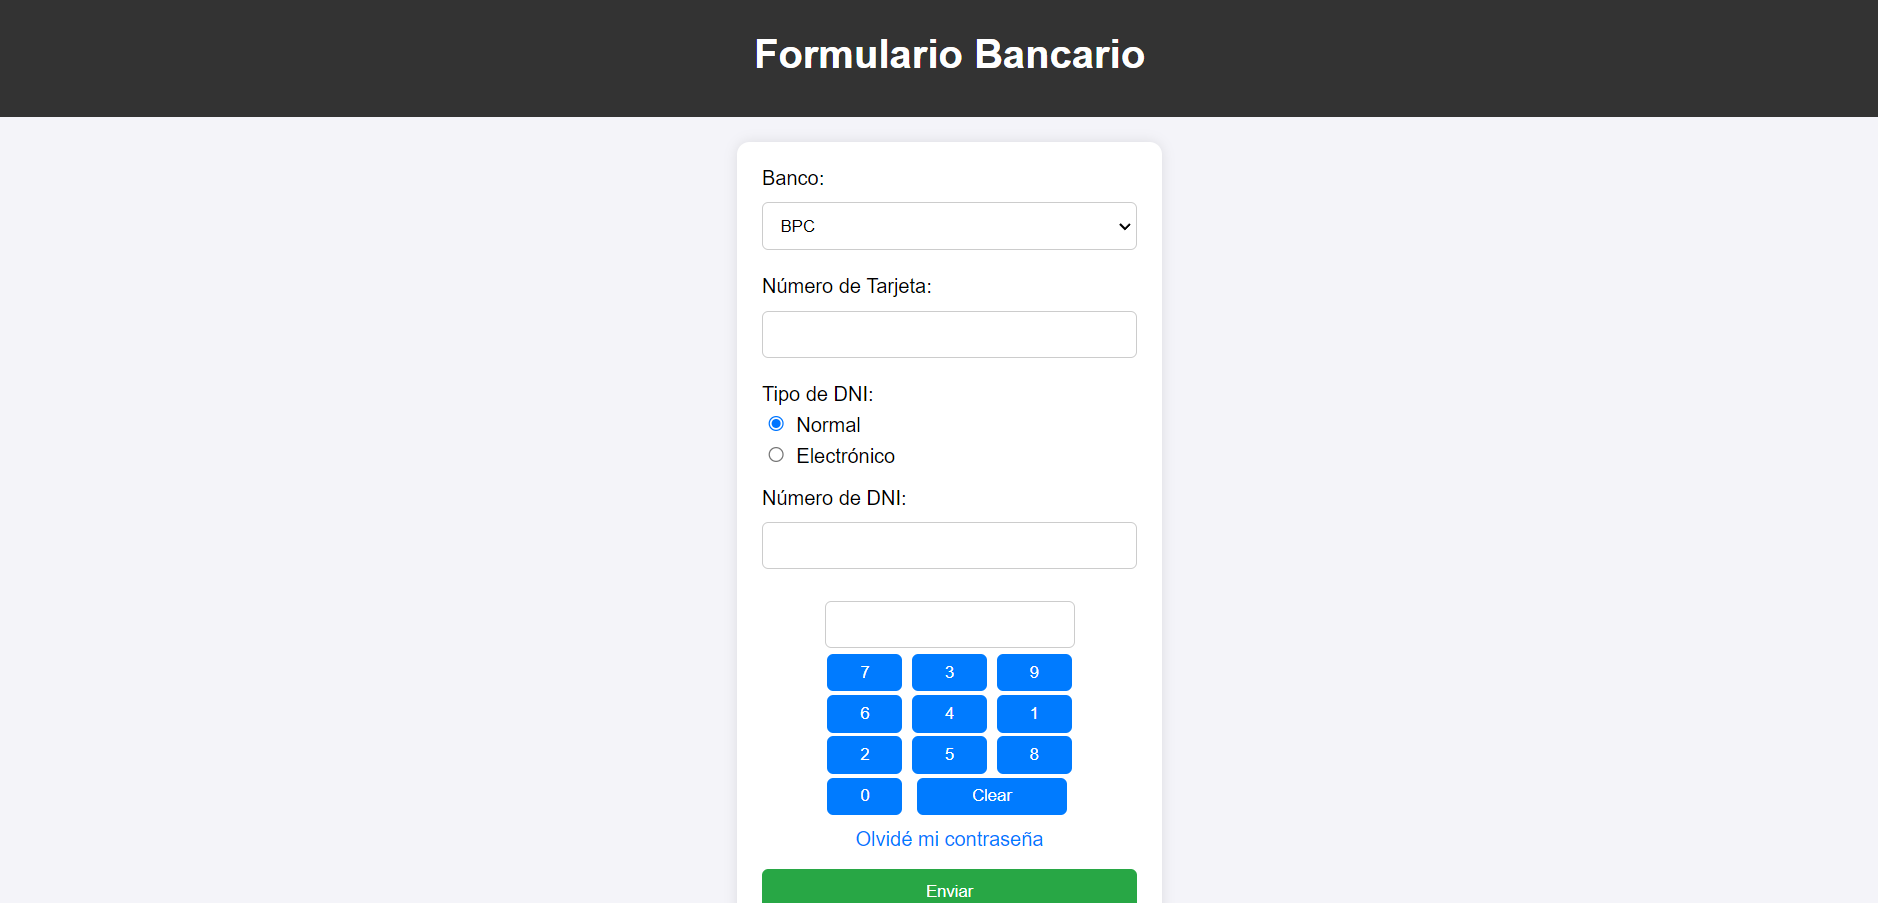
\includegraphics[width=\textwidth]{img/pag1}
            \caption{Ejecucion del Ejercicio 1}
            \label{fig:pagina}
        \end{figure}
	\end{itemize}
	
		\subsection{Ejercicio 2}
	\begin{itemize}	
		\item Documento HTML, se añadieron todos los botones que se muestran en la practica, para la pila se trato de imitar una usando una tabla
	\end{itemize}	
		
	\begin{lstlisting}[language=html,caption={Ejercicio2/index.html}][H]
<!DOCTYPE html>
<html lang="en">
<head>
    <meta charset="UTF-8">
    <meta name="viewport" content="width=device-width, initial-scale=1.0">
    <title>Calculadora</title>
    <link rel="stylesheet" href="styles.css">
</head>
<body>
    <div class="container">
        <p>Calculadora By David</p>
        <input type="text" name="text" id="in" class="in" dir="ltr">
        <div class="buttons">
            <button class="b">Del</button>
            <button class="b o">(</button>
            <button class="b o">)</button>
            <button class="b o">%</button>
            <button class="b">pi</button>
            <button class="b n">7</button>
            <button class="b n">8</button>
            <button class="b n">9</button>
            <button class="b o">/</button>
            <button class="b">sqrt</button>
            <button class="b n">4</button>
            <button class="b n">5</button>
            <button class="b n">6</button>
            <button class="b o">*</button>
            <button class="b">pow2</button>
            <button class="b n">1</button>
            <button class="b n">2</button>
            <button class="b n">3</button>
            <button class="b o">-</button>
            <button id="calc" class="big">=</button>
            <button class="b n">0</button>
            <button class="b">.</button>
            <button class="b o">%</button>
            <button class="b o">+</button>
        </div>
        <div id="stack">
            <table id="stack-table">
                <thead>
                    <tr>
                        <th>Expresion</th>
                        <th>Resultado</th>
                    </tr>
                </thead>
                <tbody>
                    <!-- Historial de calculos se inserta aca -->
                </tbody>
            </table>
        </div>
    </div>
    <script src="script_ejercicio_02.js"></script>
</body>
</html>
	\end{lstlisting}
\begin{itemize}	
		\item Archivo JavaScript, se divide en dos grandes partes: Ingresar los datos a la pantalla y procesar la pila.
	\end{itemize}	
		
	\begin{lstlisting}[language=html,caption={Ejercicio2/scriptejercicio02.js}][H]
console.log("Conexion exitosa");
var input = document.getElementById("in");

var basic = document.querySelectorAll(".b");
basic.forEach(b => {
    b.addEventListener('click', function() {
        console.log("click", b.textContent);
        input = document.getElementById("in");
        if (b.textContent === "Del") {
            input.value = input.value.slice(0, -1);
        } else if (b.textContent === "pi") {
            input.value += Math.PI;
        } else if (b.textContent === "sqrt") {
            input.value += "Math.sqrt(";
        } else if (b.textContent === "pow2") {
            input.value += "**2";
        } else {
            input.value += b.textContent;
        }
    });
});

var calcular = document.getElementById("calc");
var stackTableBody = document.querySelector("#stack-table tbody");

calcular.addEventListener('click', function() {
    try {
        var expression = input.value;
        var result = eval(expression);
        input.value = result;
        
        var newRow = stackTableBody.insertRow(0); 
        var cellExpression = newRow.insertCell(0);
        var cellResult = newRow.insertCell(1);
        cellExpression.textContent = expression;
        cellResult.textContent = result;
        input.value = "";
    } catch (error) {
        alert("Error, expresion incorrecta");
        input.value = "";
    }
});
	\end{lstlisting}
	\begin{itemize}	
		\item Imagen de la pagina.
		\begin{figure}[H]
            \centering
            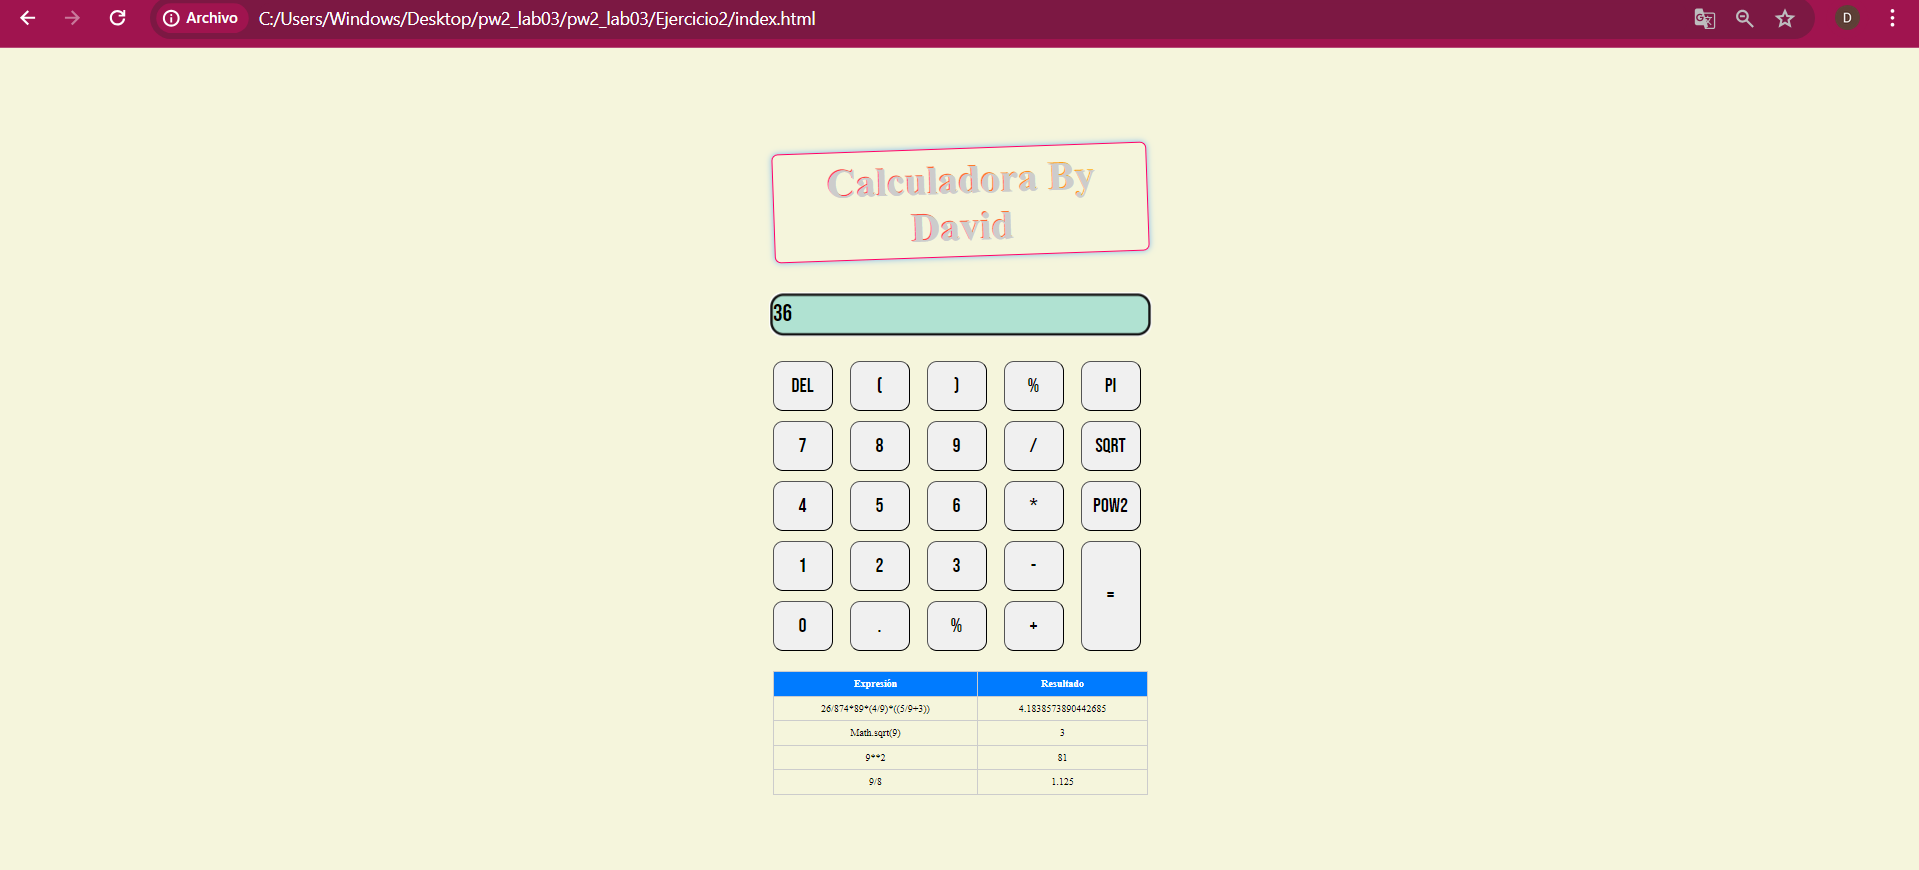
\includegraphics[width=\textwidth]{img/pag2}
            \caption{Ejecucion del Ejercicio 2}
            \label{fig:pagina}
        \end{figure}
	\end{itemize}
	
		
		\subsection{Ejercicio 3}
	\begin{itemize}	
		\item Documento HTML, se divide en dos, una ventana para escoger la dificultad del juego, cuya logica sera implementada con "display:none", y el area de juego denotada por la clase "field", posee mensajes indicando varios parametros utiles como la palabra, el canva y al final se añade un elemento para mostrar las vidas, esto a modo de practica.
	\end{itemize}	
		
	\begin{lstlisting}[language=html,caption={Ejercicio3/index.html}][H]
<!DOCTYPE html>
<html lang="en">
<head>
    <meta charset="UTF-8">
    <meta name="viewport" content="width=device-width, initial-scale=1.0">
    <link rel="stylesheet" href="styles.css">
    <title>El ahorcado!</title>
</head>
<body>
    <div id = "menu-inicial" class="menu-inicial">
        <p>Bienvenido al juego del ahorcado</p>
        <ol>
            <li>El juego comienza con una palabra secreta que debe ser adivinada.</li>
            <li>El jugador intenta adivinar la palabra proponiendo letras, una a la vez.</li>
            <li>Si la letra propuesta esta en la palabra secreta, se revela en su posicion correspondiente.</li>
            <li>Si la letra propuesta no esta en la palabra secreta, se agrega una parte del dibujo del ahorcado.</li>
            <li>El juego continua hasta que:
                <ul>
                    <li>El jugador adivine todas las letras de la palabra (victoria), o</li>
                    <li>El dibujo del ahorcado se complete (derrota).</li>
                </ul>
            </li>
        </ol>
        <div class="options">
            <div class="diff easy">
                <p>Tamanio: 5</p>
                <p>Errores: 6</p>
                <button id="easy" onclick="diffSelection(1)">FACIL</button>
            </div>
            <div class="diff medium">
                <p>Tamanio: 8</p>
                <p>Errores: 3</p>
                <button id="medium" onclick="diffSelection(2)">MEDIO</button>
            </div>
            <div class="diff hard">
                <p>Tamanio: 12</p>
                <p>Errores: 2</p>
                <button id="hard" onclick="diffSelection(3)">DIFICIL</button>
            </div>
        </div>
    </div>

    <div class="field">
        <p class="logo">EL AHORCADO!</p>
        <p>Dificultad: <span id="diff"></span></p>
        <div class="game">
            <div class="draw">
                <canvas id="myCanvas" width="200" height="150" style="border:1px solid #000000;">
            </div>
            <p>Palabras adivinadas</p>
            <p class="word" id ="word"></p>
        </div>
        <div class="teclas">
            <button class="kw">q</button>
            <button class="kw">w</button>
            <button class="kw">e</button>
            <button class="kw">r</button>
            <button class="kw">t</button>
            <button class="kw">y</button>
            <button class="kw">u</button>
            <button class="kw">i</button>
            <button class="kw">o</button>
            <button class="kw">p</button>
            <button class="kw">a</button>
            <button class="kw">s</button>
            <button class="kw">d</button>
            <button class="kw">f</button>
            <button class="kw">g</button>
            <button class="kw">h</button>
            <button class="kw">j</button>
            <button class="kw">k</button>
            <button class="kw">l</button>
            <!-No se puede representar la letra adecuada en tex-->
            <button class="kw">n</button>
            <button class="kw">z</button>
            <button class="kw">x</button>
            <button class="kw">c</button>
            <button class="kw">v</button>
            <button class="kw">b</button>
            <button class="kw">n</button>
            <button class="kw">m</button>
        </div>
        
    </div>
    <div class="container">
        <div class="lives">
            <p>Intentos restantes <span id="lives"></span></p>
        </div>
    </div>
    
    <script src="script_ejercicio_03.js"></script>
</body>
</html>
	\end{lstlisting}
\begin{itemize}	
		\item Archivo JavaScript, al inicio se definen los arreglos de palabras para cada dificultad, luego se declaran variables globales debido a que estas se modificaran segun la dificultad.
		\item Comienza con la seleccion de dificultad, cada funcion tiene el objetivo de cambiar las variables de errores, elegir la palabra adecuada, etc. Aqui se usa la funcion onclick().
		\item Se realiza una funcion para graficar al monigote en funcion del estado del juego, se implementan intrincados metodos para buscar la forma, posicion y tamaño en canvas.
		\item Por ultimo se implementa la ya conocida modalidad del juego del ahorcado, se añaden todos las funciones necesarias para actualizar la interfaz.
		
	\end{itemize}	
		
	\begin{lstlisting}[language=html,caption={Ejercicio3/scriptejercicio03.js}][H]
//Arreglos para las palabras!

const arrEasy = [
    "manos",
    "lapiz",
    "playa",
    "campo",
    "salud",
    "fruta",
    "amigo",
    "carne",
    "huevo",
    "perro"
];

const arrMedium = [
    "elefante",
    "computar",
    "edificio",
    "hospital",
    "montanas",
    "mochilas",
    "ardillas",
    "delfines",
    "paraguas",
    "escobedo"
];

const arrHard = [
    "construccion",
    "constelacion",
    "refrigerador",
    "organizacion",
    "malentendido",
    "medioambiente"
];

var tries;
var word;
var elem;
var lives;
//obtener los botones
let menuInicial = document.getElementById("menu-inicial");
let messageDiff = document.getElementById("diff");
function diffSelection(cod){
    console.log("Se selecciono, ", cod);
    menuInicial.style.display = "none";
    if(cod == 1){
        messageDiff.innerHTML = "Facil";
        easyGame();
    }else if(cod == 2){
        messageDiff.innerHTML = "Medio";
        mediumGame();
    }else{
        messageDiff.innerHTML = "Dificil";
        hardGame();
    }
    game(tries, word, elem, lives);
}



function easyGame(){
    tries = 6;
    //elegir la palabra!
    var index = Math.floor(Math.random()*11);
    word = arrEasy[index];
    console.log("La palabra es: ", word);
    //definiendo los espacios en blanco!
    elem = document.getElementById("word");
    lives = document.getElementById("lives");
    l = "";
    s = "";
    for(var i = 0; i < 5; i++){
        s += "*";
    }
    for(var i = 0; i < tries; i++){
        l += "&#128515"
    }
    elem.innerHTML = s;
    lives.innerHTML = l;
    window.scrollBy(0,50); 
}

function mediumGame(){
    tries = 3;
    //elegir la palabra!
    var index = Math.floor(Math.random()*11);
    word = arrMedium[index];
    console.log("La palabra es: ", word);
    //definiendo los espacios en blanco!
    elem = document.getElementById("word");
    lives = document.getElementById("lives");
    l = "";
    s = "";
    for(var i = 0; i < 8; i++){
        s += "*";
    }
    for(var i = 0; i < tries; i++){
        l += "&#128515"
    }
    elem.innerHTML = s;
    lives.innerHTML = l;
    window.scrollBy(0,50); 


}


function hardGame(){
    tries = 2;
    //elegir la palabra!
    index = Math.floor(Math.random()*7);
    word = arrHard[index];
    console.log("La palabra es: ", word);
    //definiendo los espacios en blanco!
    elem = document.getElementById("word");
    lives = document.getElementById("lives");
    l = "";
    s = "";
    for(var i = 0; i < 12; i++){
        s += "*";
    }
    for(var i = 0; i < tries; i++){
        l += "&#128515"
    }
    elem.innerHTML = s;
    lives.innerHTML = l;
    window.scrollBy(0,50); 
}




//Se dibujara una fase de cada dibujo!
const canvas = document.getElementById('myCanvas');
const ctx = canvas.getContext('2d');

function drawHangman(stage) {
    ctx.clearRect(0, 0, canvas.width, canvas.height); 
    ctx.strokeStyle = 'black'; 
    ctx.lineWidth = Math.max(2, Math.floor(canvas.width / 200));
    console.log(canvas.width) 
    const scale = 0.40; //definir el tamanio del lienzo
    const startX = 20 * scale;
    const startY = canvas.height - 20 * scale;
    const headX = 200 * scale;
    const headY = 80 * scale;
    const bodyY = 110 * scale;
    const armY = 140 * scale;
    const armLeftX = 150 * scale;
    const armRightX = 250 * scale;
    const legY = 250 * scale;
    const legTopX = 200 * scale;
    const legLeftX = 150 * scale;
    const legRightX = 250 * scale;
    const legBottomY = 330 * scale;

    // Dibujar la horca
    ctx.beginPath();
    ctx.moveTo(startX, startY);
    ctx.lineTo(startX, 20 * scale);
    
    ctx.moveTo(startX - 5 , startY);
    ctx.lineTo(startX - 5, 20 * scale);

    ctx.lineTo(200 * scale, 20 * scale);
    
    ctx.lineTo(200 * scale, 50 * scale);
    ctx.stroke();
    
    //cabeza
    if (stage >= 1) {
        ctx.beginPath();
        ctx.arc(headX, headY, 30 * scale, 0, Math.PI * 2);
        ctx.stroke();
    }

    //linea del cuerpo
    if (stage >= 2) {
        ctx.beginPath();
        ctx.moveTo(headX, bodyY);
        ctx.lineTo(headX, 250 * scale);
        ctx.stroke();
    }

    //linea del brazo izq
    if (stage >= 3) {
        ctx.beginPath();
        ctx.moveTo(headX, armY);
        ctx.lineTo(armLeftX, 200 * scale);
        ctx.stroke();
    }

    //linea del brazo derecho
    if (stage >= 4) {
        ctx.beginPath();
        ctx.moveTo(headX, armY);
        ctx.lineTo(armRightX, 200 * scale);
        ctx.stroke();
    }

    //linea de la pierna izq
    if (stage >= 5) {
        ctx.beginPath();
        ctx.moveTo(legTopX, legY);
        ctx.lineTo(legLeftX, legBottomY);
        ctx.stroke();
    }

    //linea de la pierna der
    if (stage >= 6) {
        ctx.beginPath();
        ctx.moveTo(legTopX, legY);
        ctx.lineTo(legRightX, legBottomY);
        ctx.stroke();
    }
}
drawHangman(0);

function game(intentos, palabra, texto, vidas) {
    let totalTries = intentos;
    
    console.log("Intentos: ", intentos);
    console.log("palabra: ", palabra);
    console.log("texto: ", texto);
    console.log("vidas: ", vidas);

    let progreso = texto.textContent.split('');

    function actualizarProgreso(letra) {
        let encontrado = false;
        for (let i = 0; i < palabra.length; i++) {
            if (palabra[i] === letra) {
                progreso[i] = letra;
                encontrado = true;
            }
        }
        return encontrado;
    }

    function haGanado() {
        return progreso.join('') === palabra;
    }

    function actualizarPantalla() {
        texto.textContent = progreso.join('');
        if(totalTries == 6){
            drawHangman(totalTries-intentos);
        }else if(totalTries == 3){
            drawHangman((totalTries-intentos) * 2);
        }else{
            drawHangman((totalTries-intentos) * 3);
        }
        
    }

    function manejarLetra(letra) {
        if (!actualizarProgreso(letra)) {
            intentos--;
            vidas.textContent = "";
            var l = "";
            for(var i = 0; i < intentos; i++){
                l += "&#128515"
            }
            vidas.innerHTML = l;
        }
        if (haGanado()) {
            alert("Has ganado La palabra era: " + palabra);
            location.reload();

        } else if (intentos === 0) {
            alert("Has perdido La palabra era: " + palabra);
            location.reload();
        }

        actualizarPantalla();
    }

    document.querySelectorAll('.kw').forEach(button => {
        button.addEventListener('click', () => {
            let letra = button.textContent;
            manejarLetra(letra);
        });
    });

    actualizarPantalla();
}
	\end{lstlisting}
	\begin{itemize}	
		\item Imagen de la pagina.
		\begin{figure}[H]
            \centering
            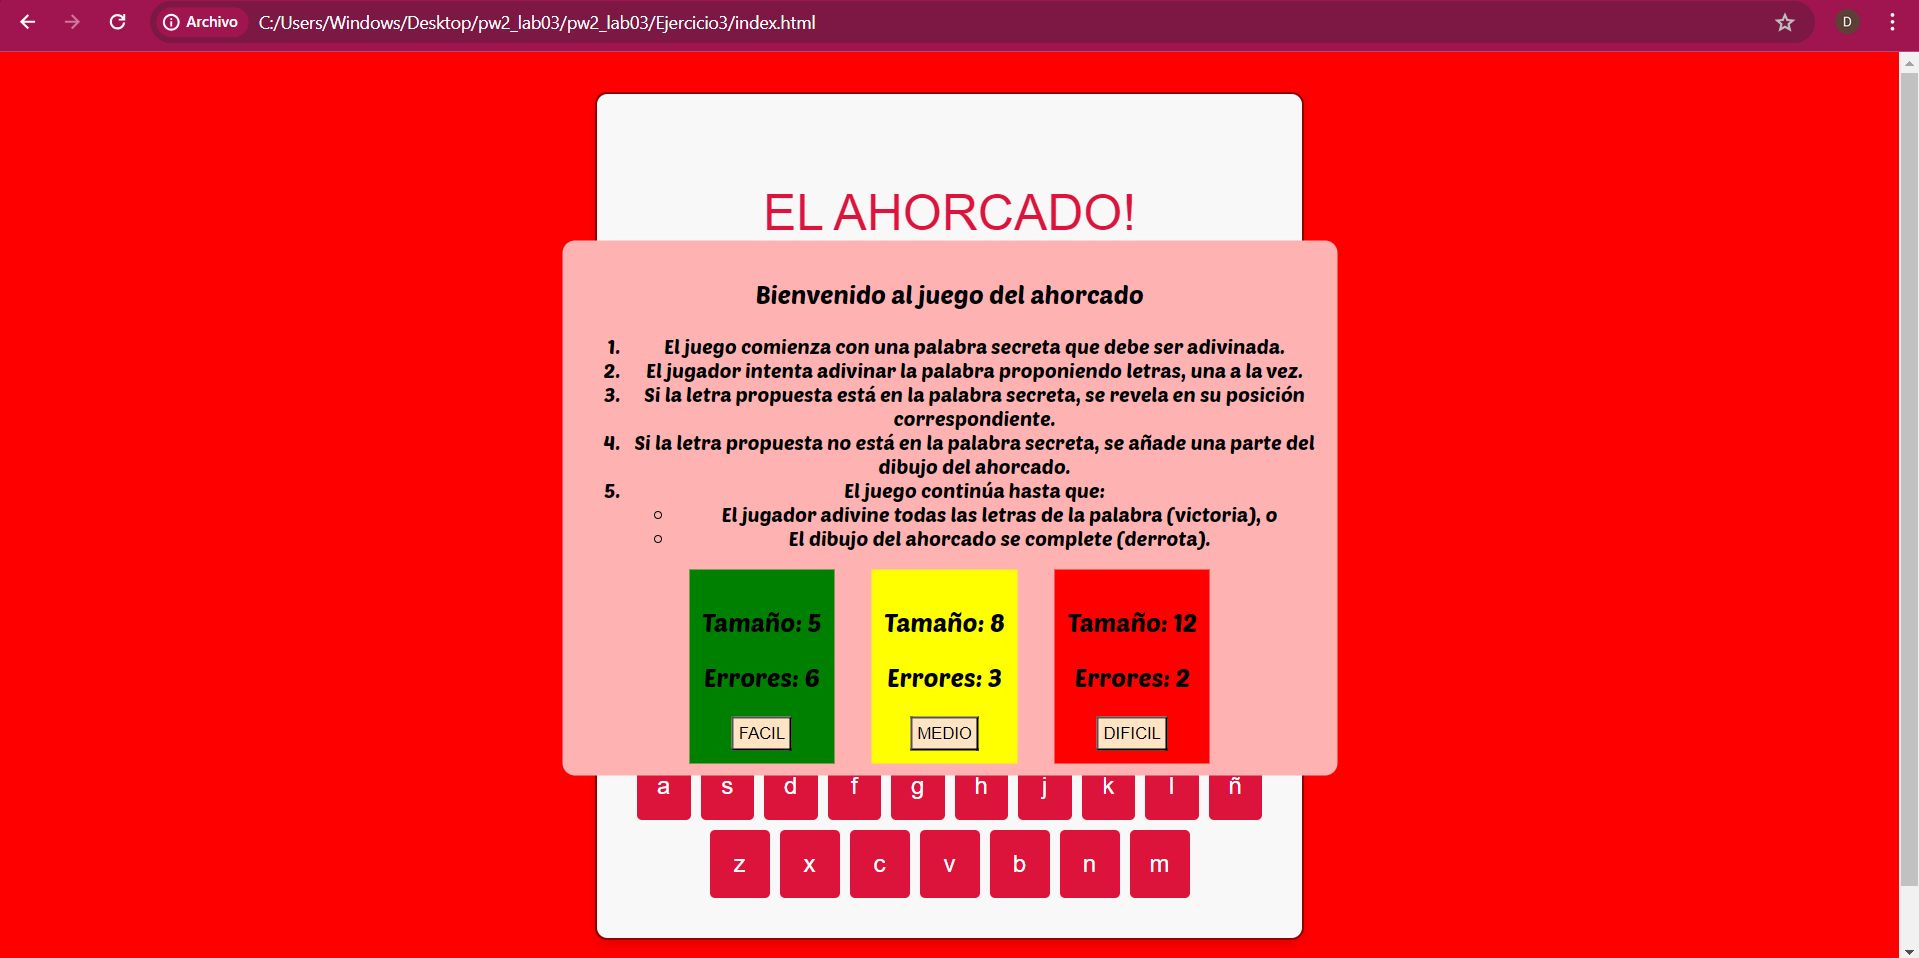
\includegraphics[width=\textwidth]{img/pag3}
            \caption{Ejecucion del Ejercicio 3}
            \label{fig:pagina}
        \end{figure}
        		\begin{figure}[H]
            \centering
            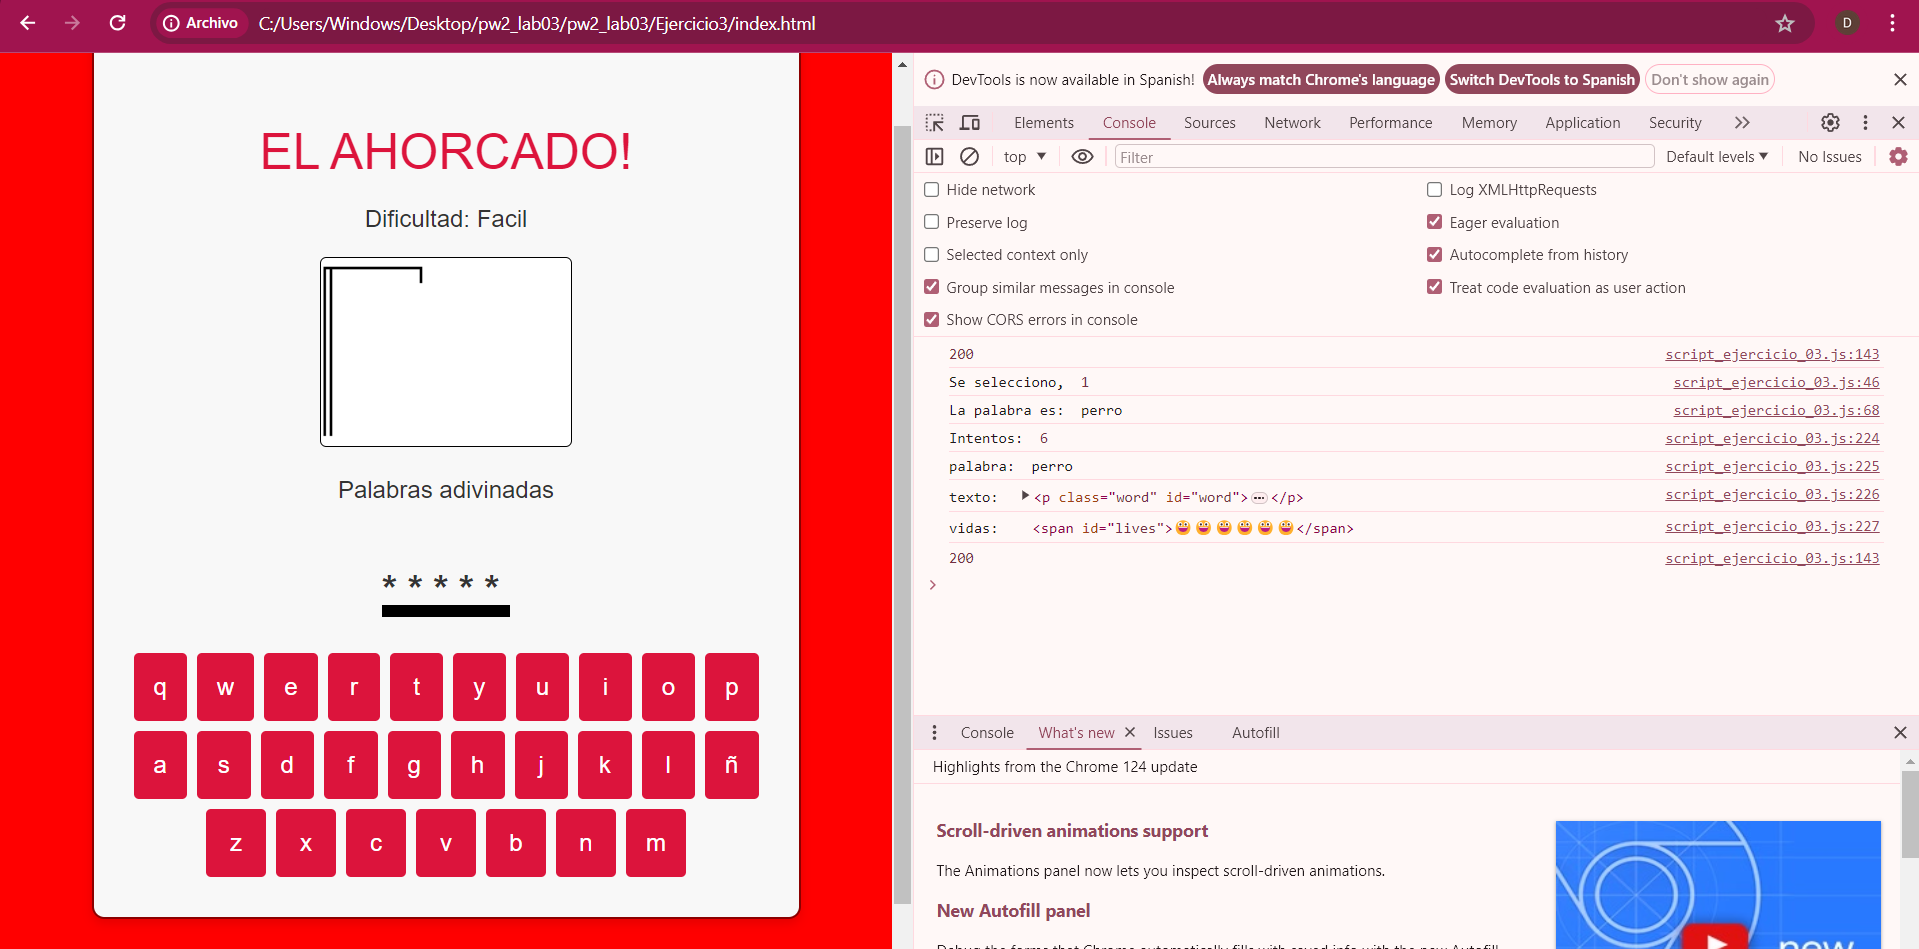
\includegraphics[width=\textwidth]{img/pag4}
            \caption{Ejecucion del Ejercicio 3}
            \label{fig:pagina}
        \end{figure}
        		\begin{figure}[H]
            \centering
            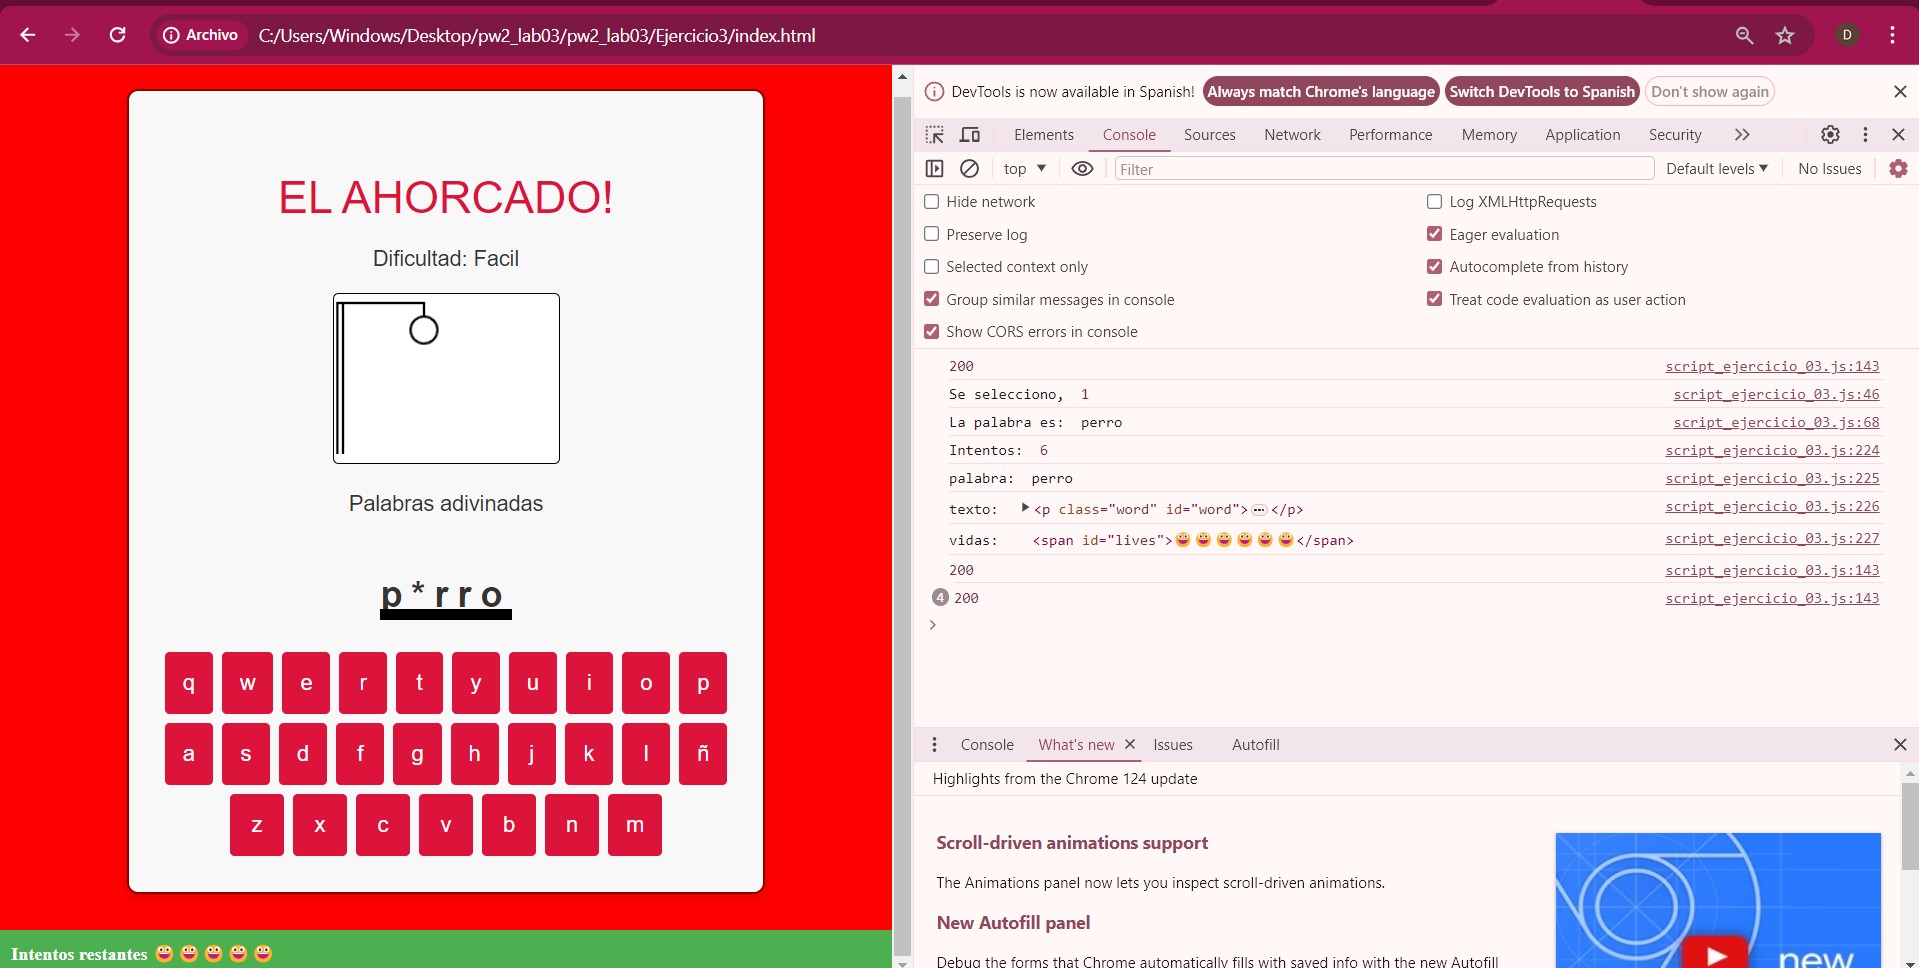
\includegraphics[width=\textwidth]{img/pag5}
            \caption{Ejecucion del Ejercicio 3}
            \label{fig:pagina}
        \end{figure}
        		\begin{figure}[H]
            \centering
            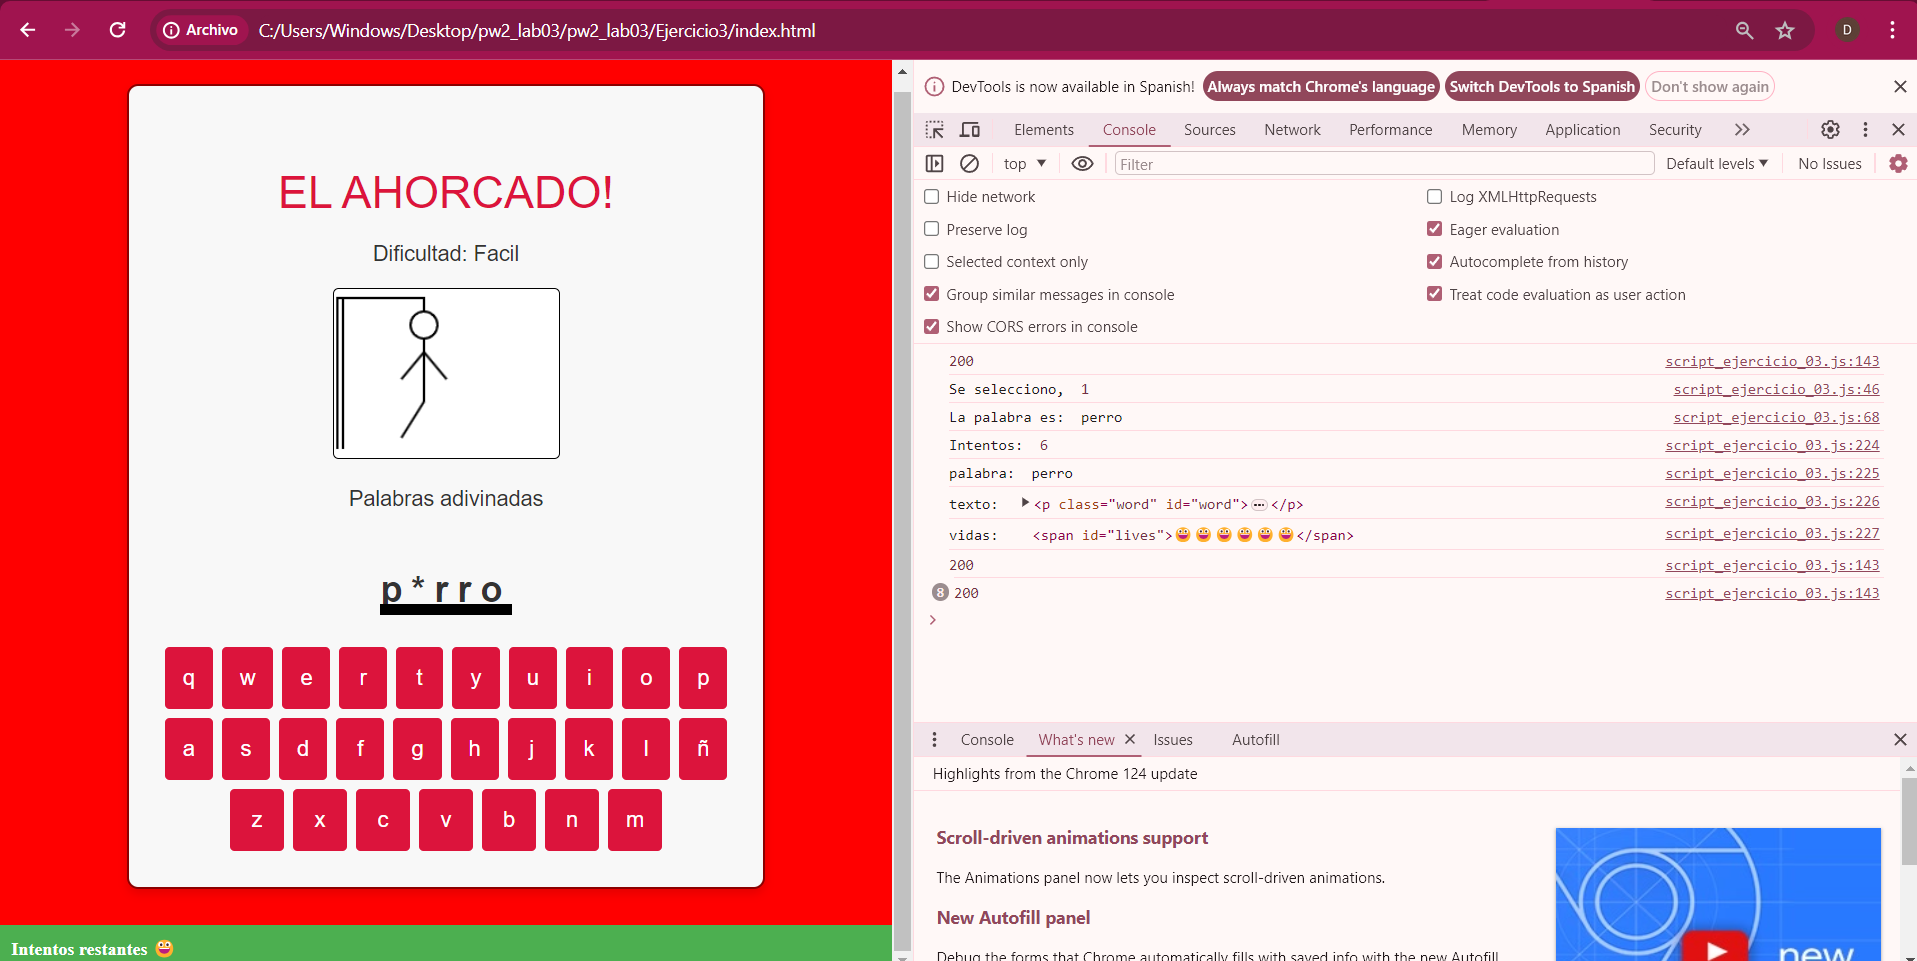
\includegraphics[width=\textwidth]{img/pag6}
            \caption{Ejecucion del Ejercicio 3}
            \label{fig:pagina}
        \end{figure}
        		\begin{figure}[H]
            \centering
            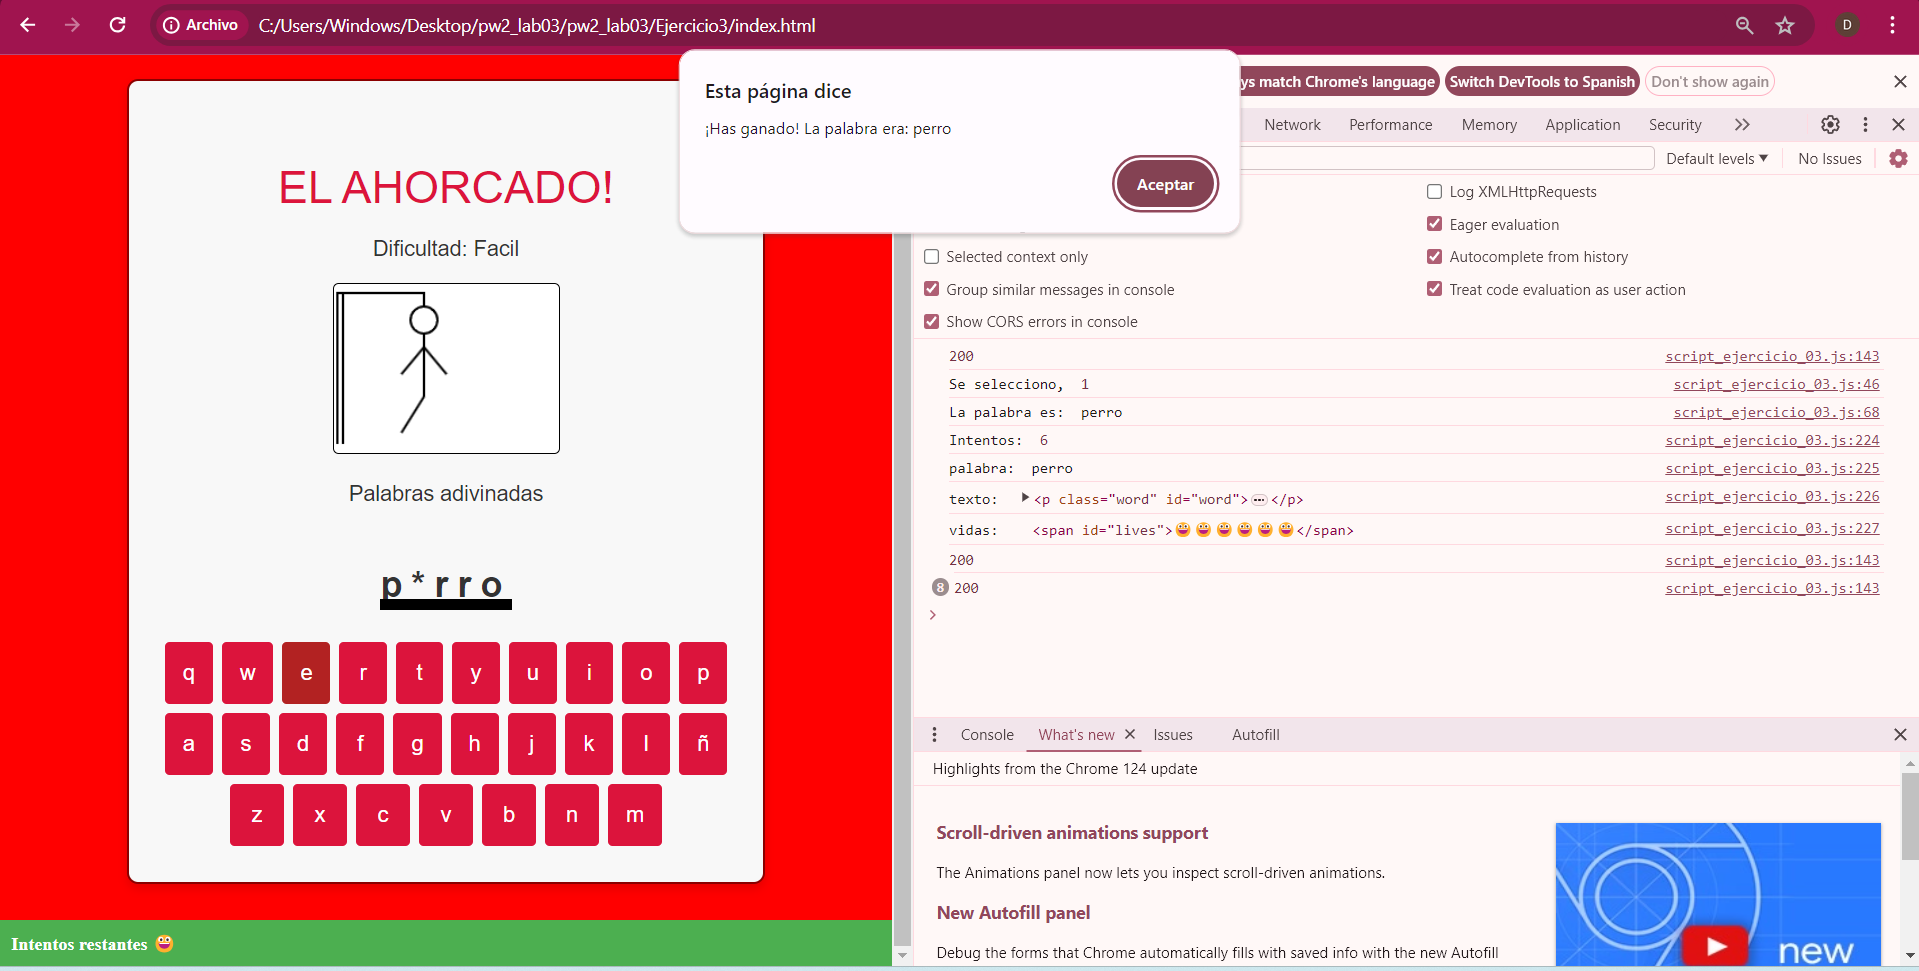
\includegraphics[width=\textwidth]{img/pag7}
            \caption{Ejecucion del Ejercicio 3}
            \label{fig:pagina}
        \end{figure}
	\end{itemize}
\section{Pregunta}
	\subsection{Explique una herramienta para ofuzcar código JavaScript.}
	\begin{itemize}	
		\item JavaScript Obfuscator es una herramienta ampliamente utilizada para ofuscar código JavaScript. Esta
herramienta transforma el código legible y entendible en una versión que es difícil de leer y comprender
para los humanos, pero que sigue siendo funcional para los navegadores y entornos de ejecución.

	\end{itemize}
		\subsection{Muestre un ejemplo de su uso en uno de los ejercicios de la tarea.}
	\begin{itemize}	
		\item Mostrando codigo ofuscado del ejercicio 2
		\begin{figure}[H]
            \centering
            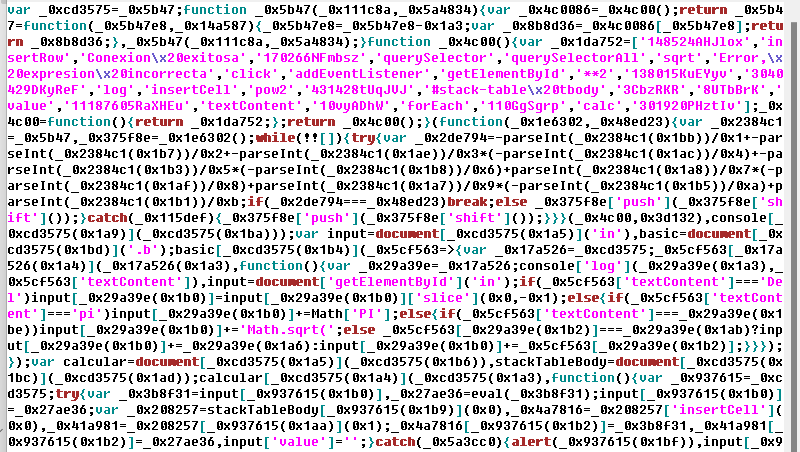
\includegraphics[width=\textwidth]{img/of}
            \caption{Codigo js del Ejercicio 2 ofuscado}
            \label{fig:pagina}
        \end{figure}
	\end{itemize}
		\subsection{Adjunte a su repositorio ambas versiones:}
	\begin{itemize}	
		\item Se implementaron los ejemplos en el repositorio
		
	\end{itemize}	

	\section{\textcolor{red}{Rúbricas}}
	
	\subsection{\textcolor{red}{Sobre el informe}}
	\begin{table}[H]
		\caption{Tipo de Informe}
		\setlength{\tabcolsep}{0.5em} % for the horizontal padding
		{\renewcommand{\arraystretch}{1.5}% for the vertical padding
		\begin{tabular}{|p{3cm}|p{12cm}|}
			\hline
			\multicolumn{2}{|c|}{\textbf{\textcolor{red}{Informe}}}  \\
			\hline 
			\textbf{\textcolor{red}{Latex}} & \textcolor{blue}{El informe está en formato PDF desde Latex,  con un formato limpio (buena presentación) y facil de leer.}   \\ 
			\hline 
			
			
		\end{tabular}
	}
	\end{table}
	
	\clearpage
	
	\subsection{\textcolor{red}{Rúbrica para el contenido del Informe y demostración}}
	\begin{itemize}			
		\item El alumno debe marcar o dejar en blanco en celdas de la columna \textbf{Checklist} si cumplio con el ítem correspondiente.
		\item Si un alumno supera la fecha de entrega,  su calificación será sobre la nota mínima aprobada, siempre y cuando cumpla con todos lo items.
		\item El alumno debe autocalificarse en la columna \textbf{Estudiante} de acuerdo a la siguiente tabla:
	
		\begin{table}[ht]
			\caption{Niveles de desempeño}
			\begin{center}
			\begin{tabular}{ccccc}
    			\hline
    			 & \multicolumn{4}{c}{Nivel}\\
    			\cline{1-5}
    			\textbf{Puntos} & Insatisfactorio 25\%& En Proceso 50\% & Satisfactorio 75\% & Sobresaliente 100\%\\
    			\textbf{2.0}&0.5&1.0&1.5&2.0\\
    			\textbf{4.0}&1.0&2.0&3.0&4.0\\
    		\hline
			\end{tabular}
		\end{center}
	\end{table}	
	
	\end{itemize}
	
	\begin{table}[H]
		\caption{Rúbrica para contenido del Informe y demostración}
		\setlength{\tabcolsep}{0.5em} % for the horizontal padding
		{\renewcommand{\arraystretch}{1.5}% for the vertical padding
		%\begin{center}
		\begin{tabular}{|p{2.7cm}|p{7cm}|x{1.3cm}|p{1.2cm}|p{1.5cm}|p{1.1cm}|}
			\hline
    		\multicolumn{2}{|c|}{Contenido y demostración} & Puntos & Checklist & Estudiante & Profesor\\
			\hline
			\textbf{1. GitHub} & Hay enlace URL activo del directorio para el  laboratorio hacia su repositorio GitHub con código fuente terminado y fácil de revisar. &2 &X &2 & \\ 
			\hline
			\textbf{2. Commits} &  Hay capturas de pantalla de los commits más importantes con sus explicaciones detalladas. (El profesor puede preguntar para refrendar calificación). &4 &X &4 & \\ 
			\hline 
			\textbf{3. Código fuente} &  Hay porciones de código fuente importantes con numeración y explicaciones detalladas de sus funciones. &2 &X &2 & \\ 
			\hline 
			\textbf{4. Ejecución} & Se incluyen ejecuciones/pruebas del código fuente  explicadas gradualmente. &2 &X &2 & \\ 
			\hline			
			\textbf{5. Pregunta} & Se responde con completitud a la pregunta formulada en la tarea.  (El profesor puede preguntar para refrendar calificación).  &2 &X &2 & \\ 
			\hline	
			\textbf{6. Fechas} & Las fechas de modificación del código fuente estan dentro de los plazos de fecha de entrega establecidos. &2 &X &2 & \\ 
			\hline 
			\textbf{7. Ortografía} & El documento no muestra errores ortográficos. &2 &X &2 & \\ 
			\hline 
			\textbf{8. Madurez} & El Informe muestra de manera general una evolución de la madurez del código fuente,  explicaciones puntuales pero precisas y un acabado impecable.   (El profesor puede preguntar para refrendar calificación).  &4 &X &2 & \\ 
			\hline
			\multicolumn{2}{|c|}{\textbf{Total}} &20 & &18 & \\ 
			\hline
		\end{tabular}
		%\end{center}
		%\label{tab:multicol}
		}
	\end{table}
	
\clearpage

\section{Referencias}
\begin{itemize}			
	\item \url{https://www.w3schools.com/js/default.asp}
\end{itemize}	
	
%\clearpage
%\bibliographystyle{apalike}
%\bibliographystyle{IEEEtranN}
%\bibliography{bibliography}
			
\end{document}